\chapter{Overview of Main VSG Topologies}

With the increasing penetration of Inverter-Based Resources (IBRs) and the
diminished involvement of Synchronous Generators (SGs) in energy generation,
existing power systems are experiencing a loss of inertia. This loss
significantly impacts two key aspects. Firstly, the absence of kinetic energy in
the system leads to a higher frequency nadir and a faster rate of change in
frequency (RoCoF), thereby affecting power quality and potentially causing the
tripping of generators \cite{alipoor2015power}.

One of the most promising solutions to address these challenges is the
implementation of Virtual Synchronous Generators (VSGs). A VSG is a control
technique applied to the switching patterns of voltage source converters (VSCs),
aiming to replicate the dynamic behavior of SGs.

% TODO: are they really active? Change the wording to avoid problem
Among the most notable research groups working on VSGs are: the VSYNC project
\cite{visscher2008vsg} under the 6th European Research Framework program, the
Virtual Synchronous Machine (VISMA) project \cite{beck2007vsm} at the Institute
of Electrical Power Engineering (IEPE) of Clausthal University of Technology in
Germany, the VSG research team at Kawasaki Heavy Industries (KHIs)
\cite{hirase2013grid}, and the Laboratory for Power Electronics and Electrical
Drives (formerly ISE Lab) at Osaka University \cite{alipoor2015power,
sakimoto2011stabilization, liu2017vsg}. In this chapter, we provide an overview
and comparison of the topologies developed by these research groups.

\section{VSYNC Project's VSG Topology}

The VSYNC project, initiated under the 6th European Research Framework program,
represents a pioneering effort in implementing virtual inertia control for
inverters. This project's system comprised an energy storage unit, a DC link,
and a power inverter with an output LCL filter connected to an AC electrical
grid \cite{visscher2008vsg}.

The control scheme incorporates a Phase-Locked Loop (PLL) and a current
reference generation circuit. The PLL is used for synchronization with the grid
frequency and for providing an angle reference for the dq transformation.
Meanwhile, the current reference generation circuit generates the reference
current for controlling the inverter's switching pattern through PWM modulation.
The overall control scheme of the VSYNC topology is illustrated in the following
image.

\begin{figure}
    \centering
    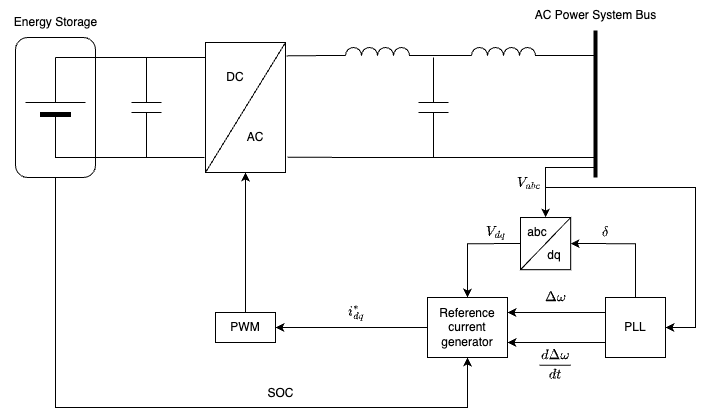
\includegraphics[width=12cm]{images/VSYNC.png}
    \caption{Overall control scheme of the VSYNC topology.}
    \label{fig:VSYNC}
\end{figure}

The current reference is calculated based on the reference active $P^*$ and
reactive $Q^*$ powers, which are calculated according to the SG swing equation
so that the overall system can emulate the SGs inertial response.
\begin{equation*}
    \begin{aligned}
        P^* &= K_{SOC}\Delta SOC + K_P \Delta\omega + K_t \frac{\Delta \omega}{dt}\\
        Q^* &= K_V \Delta V\\
        i_{d}^* &= \frac{V_d P^* - V_q Q^*}{(V_d + V_q)^2}\\
        i_{q}^* &= \frac{V_d Q^* - V_q P^*}{(V_d + V_q)^2}
    \end{aligned}
\end{equation*}

Overall, the VSYNC control scheme is a current-source, grid-supporting control
mechanism, employing a current control loop at the output terminal and using a
PLL to detect grid frequency and provide an angle reference for the dq
transformation. It is important to note that the use of a PLL can negatively
impact control performance under weak AC systems. Furthermore, the VSYNC control
scheme incorporates only the SG swing equation.

\section{IEPE's VSG Topology}

The IEPE group has proposed a VSG topology called Virtual Synchronous Machine
(VISMA), which was first implemented as a current-source-based method on a
hysteresis controlled inverter \cite{beck2007vsm,chen2011improving}, and later a
voltage-source-based method was proposed to expand its applicability to PWM
controlled inverters, which is more commonly used in the market
\cite{chen2012comparison}. The first is refered as VISMA-Method 1 and the second
is refered as VISMA-Method 2 and their overall control scheme are illustrated in
the following figures.

\newpage
\begin{figure}[h!]
    \centering
    \begin{subfigure}[b]{\textwidth}
        \centering
        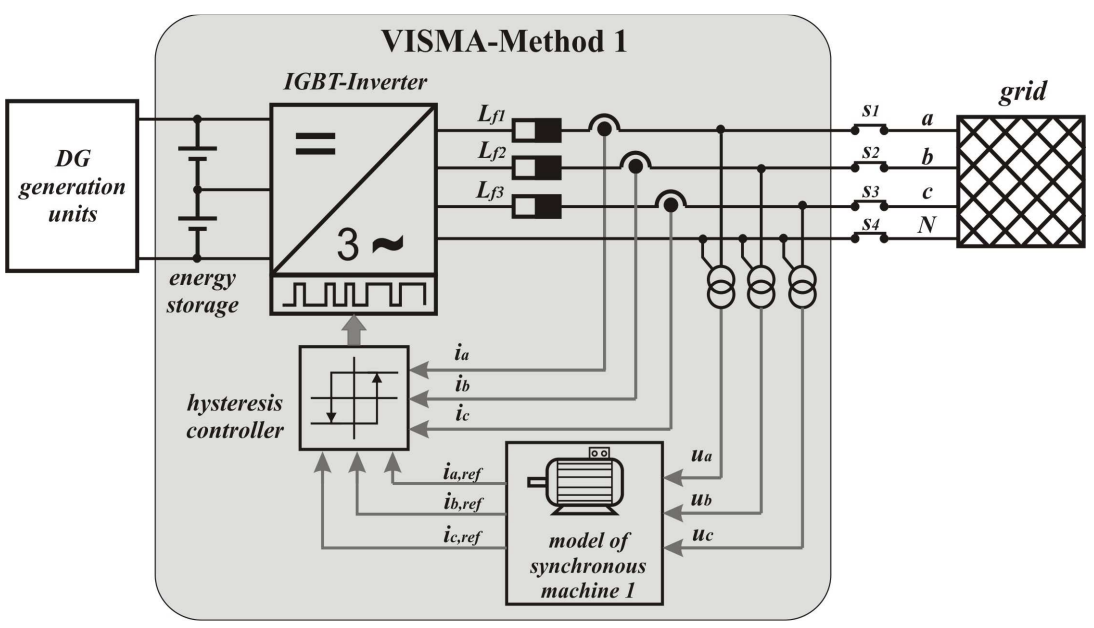
\includegraphics[width=8cm]{images/VISMA1Concept.png}
        \caption{}
        \label{fig:VISMA1Concept}
    \end{subfigure}

    \begin{subfigure}[b]{\textwidth}
        \centering
        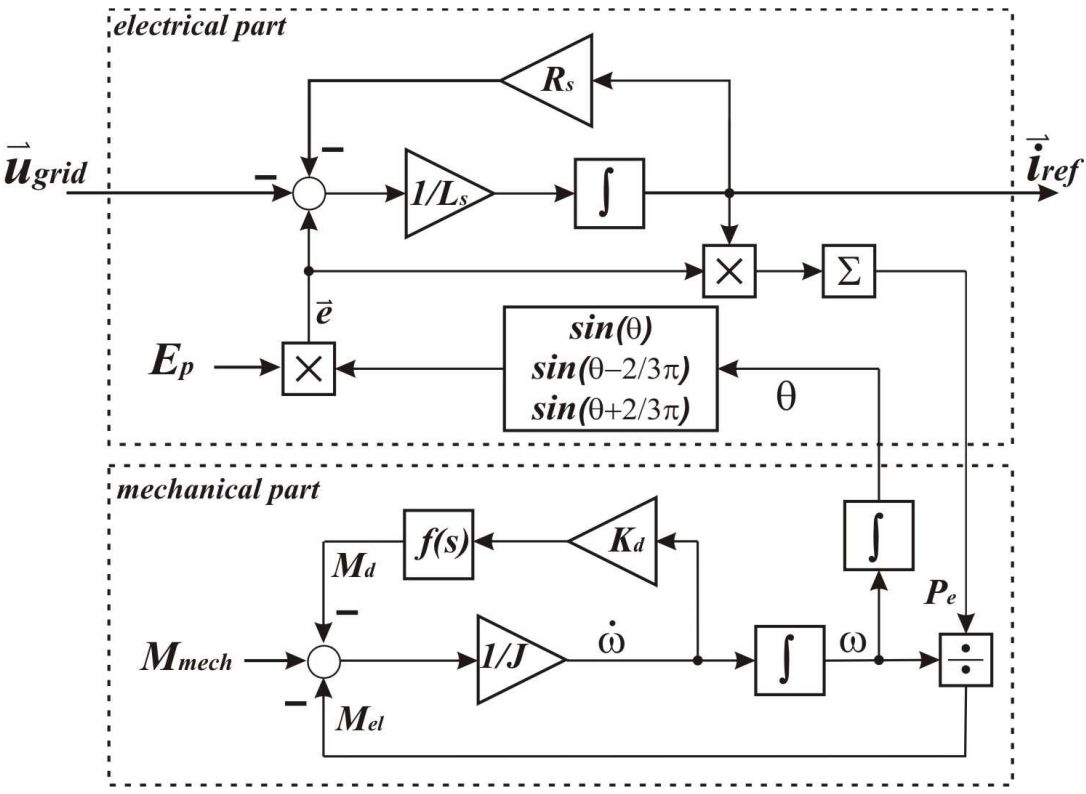
\includegraphics[width=5cm]{images/VISMA1block.png}
        \caption{}
        \label{fig:VISMA1block}
    \end{subfigure}
    \label{fig:VISMA1}
    \caption{VISMA-Method 1 (current-source-based control) \cite{chen2012comparison}. (a) Overall control scheme. (b) Model of synchronous machine 1.}
\end{figure}

\begin{figure}[h!]
    \centering
    \begin{subfigure}[b]{\textwidth}
        \centering
        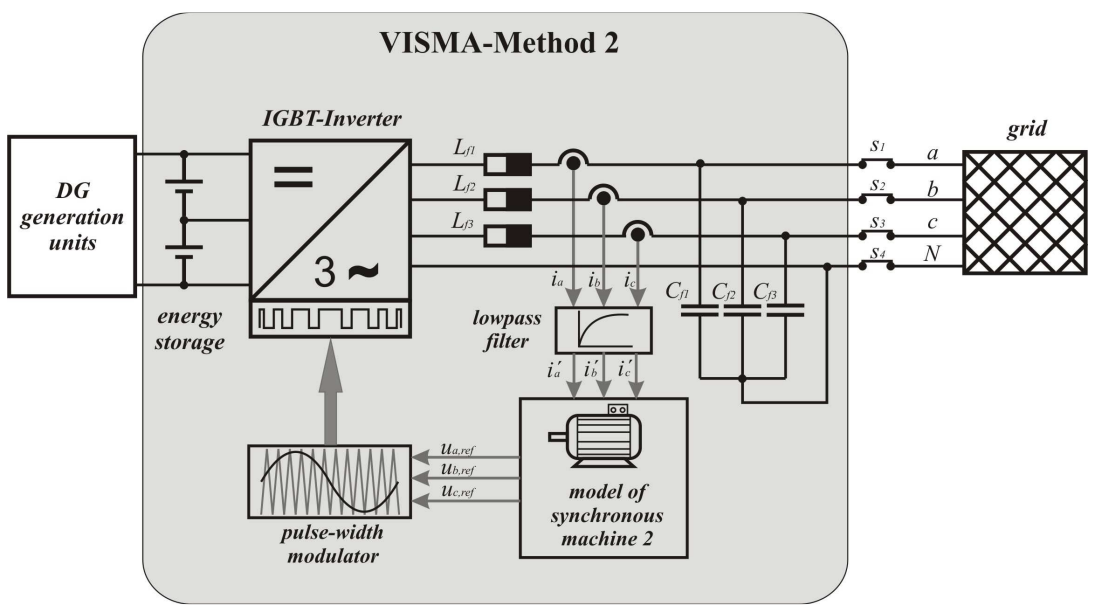
\includegraphics[width=8cm]{images/VISMA2Concept.png}
        \caption{}
        \label{fig:VISMA2Concept}
    \end{subfigure}

    \begin{subfigure}[b]{\textwidth}
        \centering
        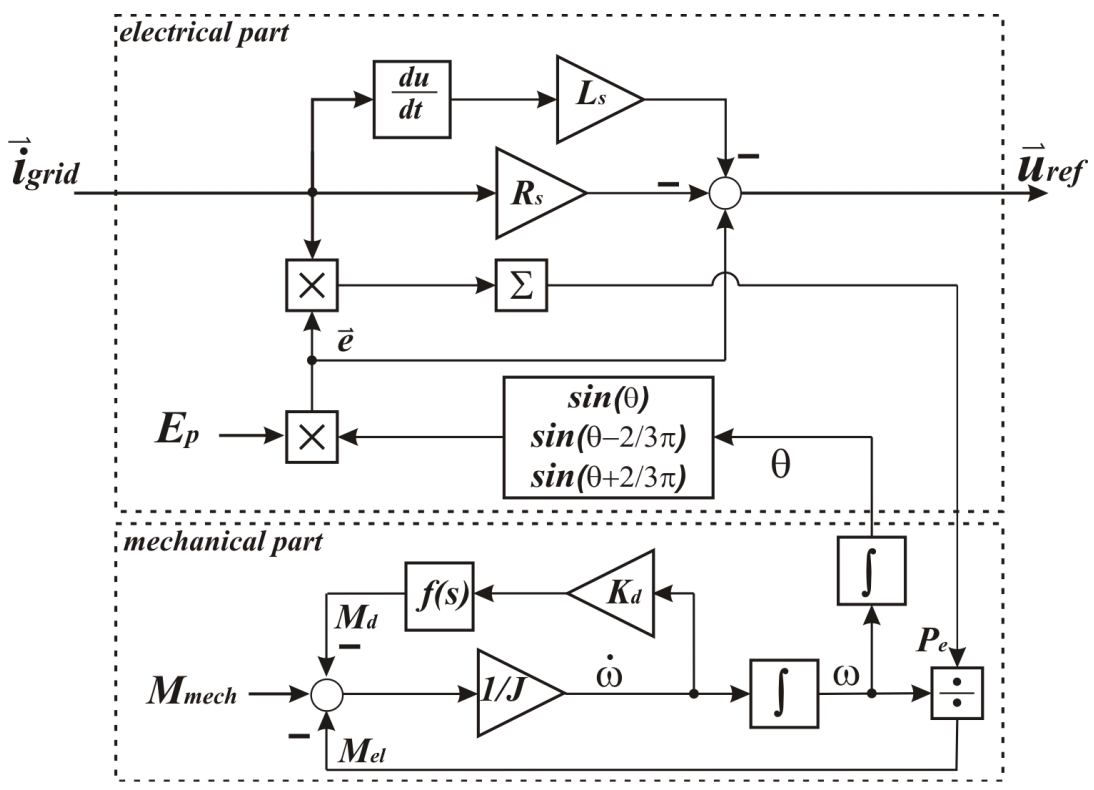
\includegraphics[width=5cm]{images/VISMA2block.png}
        \caption{}
        \label{fig:VISMA2block}
    \end{subfigure}
    \label{fig:VISMA2}
    \caption{VISMA-Method 2 (voltage-source-based control) \cite{chen2012comparison}. (a) Overall control scheme. (b) Model of synchronous machine 1.}
\end{figure}

\newpage
The VISMA-Method 1 consists in measuring the grid voltage to feed the virtual
synchronous machine algorithm, which outputs a reference current analogous to
the stator current of a SG. The virtual synchronous machine algorithm consists
of an electrical part and a mechanical part that interact with each other. The
mechanical part corresponds to the rotor dynamics of the virtual synchronous
machine, and can be represented by the following equations:

\begin{equation*}
    \begin{aligned}
        M_{mech} - M_{el} &= \frac{1}{J} \frac{d\omega}{dt} + k_d f(s) \frac{d\omega}{dt}\\
        M_{el} &= \frac{P_{el}}{\omega}\\
        \theta &= \int \omega dt
    \end{aligned}
\end{equation*}
\noindent where $J$ is the moment of inertia, $k_d$ is the mechanical damping
factor, $f(s)$ is the phase compensation term, $\omega$ is the angular speed,
$\theta$ is the angular position and $M_{el}$ and $M_{mech}$ are the electrical
and mechanical torque.

$M_{mech}$ represents the action of the virtual governor, which is simplified as
being a control input to the system. The excitation system is also simplified,
being represented by an adjustable amplitude $E_p$, resulting in the following
induced electromotive force in the virtual stator.

\begin{equation*}
    \overrightarrow{e} =
    E_p\begin{bmatrix}e_a \\e_b \\ e_c\end{bmatrix} =
    E_p\begin{bmatrix}\sin{(\theta)} \\\sin{(\theta - \frac{2\pi}{3})} \\ \sin{(\theta + \frac{2\pi}{3})} \end{bmatrix}
\end{equation*}

Then, this induced electromotive force is used with the measured grid voltage in
the electrical part of the virtual synchronous machine model to calculate the
reference current, which is then used to drive the hysteresis controlled
converter. The electrical part of the synchronous machine model is represented
by the following equations.

\begin{equation*}
    \begin{aligned}
        e_a - u_a &= i_a^{ref}R_s + L_s\frac{di_a^{ref}}{dt}\\
        e_b - u_b &= i_b^{ref}R_s + L_s\frac{di_b^{ref}}{dt}\\
        e_c - u_c &= i_c^{ref}R_s + L_s\frac{di_c^{ref}}{dt}
    \end{aligned}
\end{equation*}
\noindent where $(u_a, u_b, u_c)$ are the measured grid voltage in each line,
$R_s$ and $L_s$ are the virtual stator resistance and inductance, respectively.

The working principle of the VISMA-Method 2 is exactly the same as of the
VISMA-Method 1, with the exception that the grid current is used instead of the
grid voltage for calculating the reference signal to drive the PWM based
converter. In other words, the electrical part of the synchronous machine model
is now represented by:

\begin{equation*}
    \begin{aligned}
        e_a - u_a^{ref} &= i_a R_s + L_s\frac{di_a}{dt}\\
        e_b - u_b^{ref} &= i_b R_s + L_s\frac{di_b}{dt}\\
        e_c - u_c^{ref} &= i_c R_s + L_s\frac{di_c}{dt}
    \end{aligned}
\end{equation*}
\noindent where $(i_a, i_b, i_c)$ are the measured grid current in each line.

It is important to highlight that the VISMA topology does not require a PLL and
uses a 5th order model of a SG, comprising of two mechanical state variables
($theta$ and $\omega$) and 3 electromagnetic state variables (the stator
quantities). However, the damper and excitation windings are not taken into
consideration, and the transient and sub-transient dynamics are ignored.
Moreover, this model does not consider possible saliency effects of the rotor.

\section{KHIs' VSG Topology}
KHI has proposed a current-source-based VSG topology in the $dq$-coordinate
frame\cite{hirase2013grid}, which control diagram is illustrated in the
following image.

\begin{figure}[h!]
    \centering
    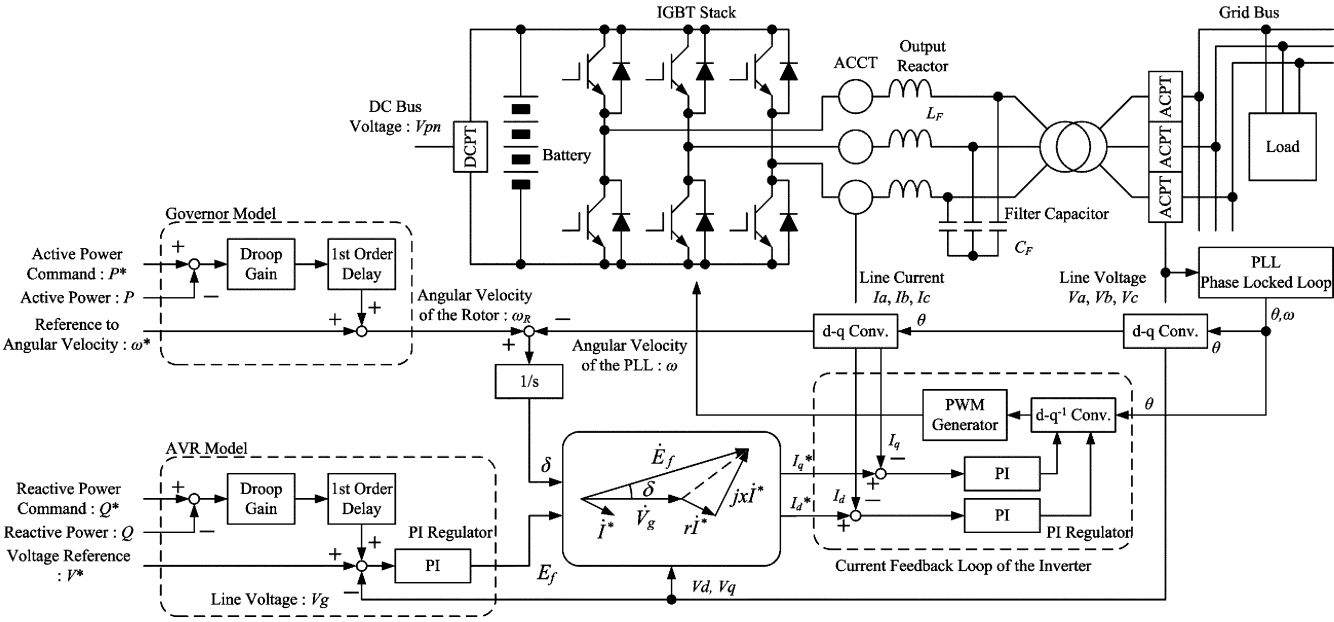
\includegraphics[width=14cm]{images/KHI.png}
    \caption{Control diagram of the VSG control developed by KHI\cite{hirase2013grid}.}
    \label{fig:KHI}
\end{figure}

In this model, the authors use phasor diagrams to express the relationship
between the phase voltage and line currents of the virtual generator, thus
ignoring the electrical dynamics. Moreover, the virtual generator is assumed to
be cylindrical, with the same synchronous reactance on the direct and quadrature
axes.

The model is composed of four main components: a PLL, an AVR, a virtual
governor, a virtual generator model, and a current feedback loop. The PLL is
used to detect the angular speed and angle of the grid side voltage of the
inverter's output filter, which is used in the $dq-$transformations.

The output active and reactive powers are also measured, and they are in the
virtual governor and AVR models to generate, respectively, the angular speed of
the virtual rotor, and the internal electromotive force. The virtual governor
and AVR models are simple PI controllers for active and reative power
regulation.

The outputs from the virtual governor and AVR are then used to compute the
reference current, which then passes through a current feedback loop to generate
the reference signal for the PWM modulation.

\section{ISE Lab's VSG Topology}
The Laboratory for Power Electronics and Electrical Drives (formely ISE Lab) at
Osaka University, which consists in emulating the SG swing equation
\cite{sakimoto2011stabilization,shintai2012reactive}. The following image
describes the block diagram of the Ise Lab's VSG topology.

\begin{figure}[h!]
    \centering
    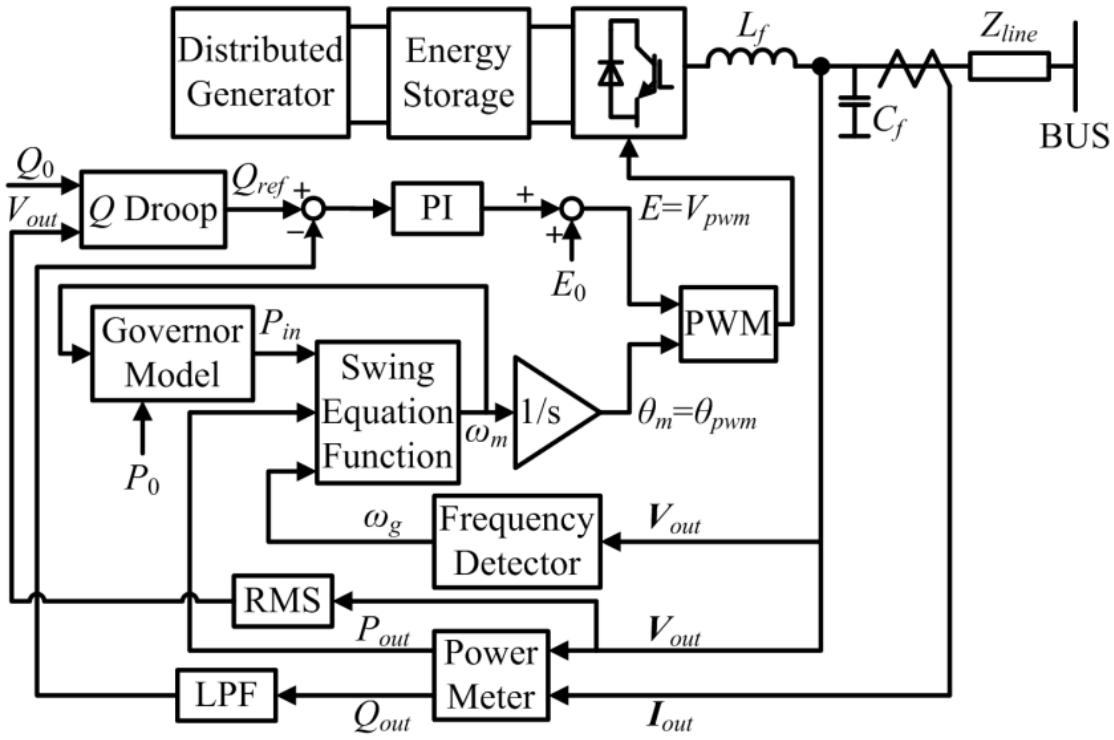
\includegraphics[width=14cm]{images/ISE.png}
    \caption{Control diagram of the VSG control developed by ISE Lab\cite{liu2016studies}.}
    \label{fig:ISE}
\end{figure}

This model consists in measuring the output current and voltage, which are then
used to compute the output active and reactive powers. The Frequency Detector
block corresponds to a PLL that is used to measure the bus frequency $\omega_g$
which is used to compute the virtual rotor frequency through the swing equation:

\begin{equation*}
    P_{in} - P_{out} = J\omega_m \frac{d\omega_m}{dt} + D(\omega_m - \omega_g)
\end{equation*}

The rotor frequency is used as a reference for the governor model and the PWM
inverter. Both the governor model and the Q Droop block are droop controllers
creating linear droop control law between active power and frequency, and
between reactive power and voltage, respectively.

It is important to highlight that no inner current or voltage loop is adopted in
this control scheme, so that the filter reactance is analogous to the stator
reactance of the VSG. Moreover, this VSG control can be classified as a
voltage-source-based grid-forming control.

However, 

\section{Synchronverter}


% Classification according to Current Controlled or Voltage Controlled
% Explanation of main topologies of VSG
% VSG used in this thesis
% Comparison of topologies in terms of reference model